%to build: "pdflatex report.tex"

%\documentclass[journal]{IEEEtran}
\documentclass{article}
\usepackage{amsmath}
\usepackage{listings}
\usepackage{graphicx}
\usepackage{multicol}
\usepackage{wrapfig}
\graphicspath{./imgs/}
\DeclareGraphicsExtensions{.pdf, .jpeg, .png}
\usepackage{geometry}
\geometry{a4paper, portrait, margin=1in}

\newcommand{\includecode}[2][c]{\lstinputlisting[caption=#2, escapechar=, language=#1]{#2}}
 
\hyphenation{op-tical net-works semi-conduc-tor}
\begin{document}

\title{Computational Physics Midterm Project}
\author{
Austin~F.~Oltmanns
\and
Noah~Seekins
}

\maketitle

% As a general rule, do not put math, special symbols or citations
% in the abstract or keywords.
\begin{abstract}
The goal of this project was to simulate lighting through a scene using ray-tracing and a pinhole camera to view said scene.
Ray-tracing techniques are explored for the purpose of rendering 3d scenes which contain meshes made of
triangular sections of planer surfaces. Linear algebra techniques are used to obtain computationally 
efficient methods  for detecting the intersections of the rays with the triangular meshes within the scene.
It is shown that shadows are simulated using this method, which is an improvement 
from rendering techniques previously explored in the class.
\end{abstract} 

\section{Introduction}
%\IEEEPARstart{T}{his}
This midterm assignement required students to design and develop a simulation of a physical phenomenon 
of their choosing. Our group chose to explore ray-tracing because we felt it aligned fairly closely with the 
material presented in class thus far and also presented a complex enough subject to warrent exploration.
The system implemented shows a triangular section casting a shadow onto a ground plane from light sources
present above the triangular surface (above meaning in the +Z direction of the world's coordinates).

To perform this experiment, light rays are traced starting from their end point inside the camera, out through
a pinhole, reflected a number of times off of the world, and back to either a light source or found to not 
reach a light source. In this particular simulation, only two reflections maximum are used.

For simplicity, real world units have been disregarded in an effort to keep the numbers used in the simulation from 
becoming very large or small (which can affect the stability of the simulation).
Each aspect of the simulation will be described in detail below and the code is attached as an appendix to this report.

\section{Ray Generation}
\subsection{Description}
%ORDER
The first step is to determine the end point of each ray inside the camera. These end points correspond to 
pixels displayed on the screen and the color of each pixel is an average of the color of each ray which ends
at that point. This implies that for each pixel, there must be a sufficient number of rays which terminate
at that point. To determine each of these rays' origin points and directions in the world coordinate system,
a transform from the imaging plane of the camera (the "film") to the world is created based on parameters from the camera.

%%%
%Figure of plane with vectors pointing to the pinhole
%%%
\begin{figure}[!t]
\centering
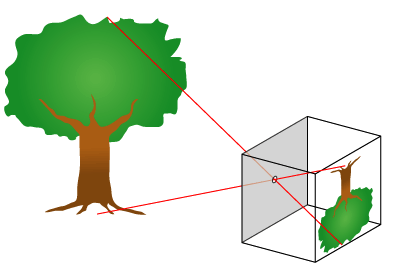
\includegraphics[width=3.5in]{./imgs/Pinhole-camera}
\caption{The rays are shown in this figure as the red lines. Note how each ray passes through the pinhole
of the camera from the imaging plane and into the world. (Public Domain)}
\label{fig:pinhole}
\end{figure}

Fig.~\ref{fig:pinhole} shows two rays begining (ending) at the imaging plane and passing through the pinhole
of the virtual camera. What is not shown is how the rays reflect off of objects in the world to arrive
 (or not arrive) at light sources.

\subsection{Implementation}
If the axes which define the coordinates system with its origin at the pinhole of the camera and rotated 
to point in a direction as a camera does are written as vectors described in world coordinates, then a 
transform from camera coordinates to world coordinates can be constructed as follows.


The first step is to determine the translation matrix which would translate the coordinates of a point in world
coordinates to a set of coordinates which would be defined by the camera if it had no rotation relative to the world's
coordinate system. This matrix is denoted $T$ in Eqn.~\ref{eqn:trans}. 

\begin{equation}
T=
  \begin{bmatrix}
   1 & 0 & 0 & X_0 \\
   0 & 1 & 0 & Y_0 \\
   0 & 0 & 1 & Z_0 \\
   0 & 0 & 0 & 1
  \end{bmatrix}
  \label{eqn:trans}
\end{equation}


The second step is to find the rotation matrix 
which would transform the coordinates of a particle in world coordinates to that of the camera if it were located at 
the origin but rotated. This matrix is denoted $R$ in Eqn.~\ref{eqn:rot}.

\begin{equation}
R=
  \begin{bmatrix}
   U_x & V_x & W_x & 0 \\
   U_y & V_y & W_y & 0 \\
   U_z & V_z & W_z & 0 \\
   0 & 0 & 0 & 1
  \end{bmatrix}
  \label{eqn:rot}
\end{equation}

Finally, by combining these operations, the
final transformation matrix (denoted $M$ in Eqn.~\ref{eqn:total}) is obtained as the product of the two prior transforms
and points/particles described in world coordinates can be described in camera coordniates by applying Eqn.~\ref{eqn:doit}.

\begin{equation}
M = RT
\label{eqn:total}
\end{equation}

\begin{equation}
\begin{bmatrix}
  x' \\
  y' \\
  z' \\
  1
\end{bmatrix}
  = M
\begin{bmatrix}
  x \\
  y \\
  z \\
  1
\end{bmatrix}
\label{eqn:doit}
\end{equation}

\begin{figure}[!b]
\centering
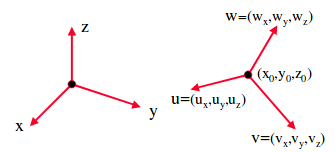
\includegraphics[width=3.5in]{./imgs/axes}
\caption{World and camera axes together. Camera axes have been defined with reference to the world axes.}
\label{fig:axes}
\end{figure}

Now that this transform is available, it is trivial to take points from a plane in camera coordinates and transform 
them to points in world coordinates. These points form the origin's of the rays from the camera. To find the direction
of each vector, some geometric manipulations are done. The following section of code demonstrates this.

\begin{lstlisting}[language=C]
  for (int row=0; row<numRaysRows; row++)
  {
     for (int col=0; col<numRaysCols; col++)
     {
        //find point on imaging plane in camera coord
        double filmy = row * raydistance - centery;
        double filmx = col * raydistance - centerx;
        double filmz = -cam.zoom;
        //take (normal point - film point) and normalize to get unit direction 
        // vector in camera coord
        double magnitude = sqrt(filmy * filmy + filmx * filmx + cam.zoom*cam.zoom);
        
        double udvU = -filmy/magnitude;
        double udvV = -filmx/magnitude;
        double udvW = cam.zoom/magnitude;
        //apply inverse tf to film point to get origin in world coord
        gsl_matrix_set(originPoint, 0,0, filmx);
        gsl_matrix_set(originPoint, 1,0, filmy);
        gsl_matrix_set(originPoint, 2,0, filmz);
        gsl_matrix_set(originPoint, 3,0, 1);

        gsl_blas_dgemm(CblasNoTrans, CblasNoTrans, 1, inverseTransform, 
                       originPoint, 0, result);
        
        rays[row + numRaysRows * col].origin[0] = gsl_matrix_get(result, 0,0);
        rays[row + numRaysRows * col].origin[1] = gsl_matrix_get(result, 1,0);
        rays[row + numRaysRows * col].origin[2] = gsl_matrix_get(result, 2,0);
        //apply inverse tf to unit direction vector to get udv in world coord
        gsl_matrix_set(unitDirectionVector, 0,0, udvU);
        gsl_matrix_set(unitDirectionVector, 1,0, udvV);
        gsl_matrix_set(unitDirectionVector, 2,0, udvW);
        gsl_matrix_set(unitDirectionVector, 3,0, 1);

        gsl_blas_dgemm(CblasNoTrans, CblasNoTrans, 1, renderman.rot, 
                       unitDirectionVector, 0, result);

        rays[row + numRaysRows * col].direction[0] = gsl_matrix_get(result, 0,0);
        rays[row + numRaysRows * col].direction[1] = gsl_matrix_get(result, 1,0);
        rays[row + numRaysRows * col].direction[2] = gsl_matrix_get(result, 2,0);
     }
  }
\end{lstlisting}

\section{Plane Generation}
\subsection{Description}
The second step in the process of creating an accurate simulation is to create a way to model the triangular planes
that will allow for interaction with the rays in the world. Each triangular plane is described using three vertices
which outline the section of a given plane that is inside the given triangle. Each plane also needed several properties
outlining the color and material of the given plane.
\subsection{Implementation}
\begin{lstlisting}[language = C]
  typedef struct triangle_S
  {
    double v0[3], v1[3], v2[3]; //vertices of triangle in world coord
    double reflectionIndex; // 0 to 1 on how dispersive(0)/reflective(1) surface is
    double lightSource; //how much light the surface produces (0 to 1)
    double hue, sat; //hue and sat are from material
    
  } triangleSurface;
\end{lstlisting}
We utilized a structure format in order to easily make and keep track of our surface code, which is outlined above.
v0, v1, and v2 are the vertices of the triangle in our coordinate system, reflectionIndex describes how reflective
a given triangular surface is, lightscore describes how much light a given triangular section gives off, making
it useful for creating light sources, and the hue and saturation, which control how bright and vibrant the colors of
the reflected light are. The structure format  allowed us to include this code in our other code sections, which
allowed us to use these structures to store all the data we needed to generate a triangular plane in all of our
other files.
\section{Ray interaction with World}
The second step in the process of creating an accurate simulation is to allow the rays to interact with
the world, specifically, the triangular planar sections that we generated using the triangular structure
code that we created in a structure (the code for which we included at the beginning of the file). The first
issue we needed to tackle was figuring out whether the given ray intersected the given plane at all.
\begin{lstlisting}[language=C]
  double dotProduct(double E1[3], double E2[3]){
    double result=0;
    for (int i=0; i<3; i++){
      result +=E1[i]*E2[i];
    }
    return result;
  }
  void crossProduct(double a[3], double b[3], double * result)
  {
    
    result[0] = a[1]*b[2] - a[2]*b[1];
    result[1] = a[2]*b[0] - a[0]*b[2];
    result[2] = a[0]*b[1] - a[1]*b[0];
  }
\end{lstlisting}
The very first thing we did was to create functions for our cross products and our dot products, as both were
mathematical tools that we would need to use multiple times throughout the process of both determining whether
or not the particle hit the plane, but also to how the particle reflected off of the plane. In order to take the dot
product, we multiplied the corresponding members of two vectors (in our code represented by arrays), and added them all
together, which corresponds to taking the dot product of two vectors manually. The cross products were a bit tougher, but
we utilized the standard method for taking a 3 by 3 determinant (and thereby taking the cross product) to get each member
of the array, and each element of the resultant vector.
\begin{lstlisting}[language=C]
  for(int i=0; i<3; i++){
    edge0[i]=(surf->v0[i])-(surf->v1[i]);
    edge1[i]=(surf->v1[i])-(surf->v2[i]);
    edge2[i]=(surf->v2[i])-(surf->v0[i]);
  }
  crossProduct(edge0,edge1,N);
\end{lstlisting}
We started the process of calculating the intersection of the ray and the planes  by outlining the edge lengths of
the space, and taking the cross productof two of the edges to get the normal vector of the plane. We do this, as both
the normal vector and the edges will be useful later for describing the plane's direction.
\begin{lstlisting}[language=C]
  double denom = dotProduct(N, ray->direction);
  if (denom > 1e-6){
    double numer[3];
    for (int i=0;i<3;i++){
      p0l0[i]=surf->v0[i] - ray->origin[i];
    }
    t = dotProduct(p0l0,N)/denom;
  }
  else{
    return MISS;
  }
\end{lstlisting}
\begin{equation}
  \hat{A}\dot\hat{B}=|\hat{A}||\hat{B}|cos(\Theta)
  \label{DPE}
\end{equation}
In this next section of the code, we make use of the normal vector that we found earlier in order to calculate the
dot product between the direction vector of the ray and the normal. This is essentially calculating how paralell the
two vectors are along with multiplying their magnitudes, as though the way we do this in our code is by multiplying and
adding the elements of the two vectors which we wish to manipulate, another way to describe a cross product is given in
equation (\ref{DPE}). After this, we check to see that this value is not very small, as if it were, that would mean that
the plane and the ray are perpandicular, or so very nearly perpandicular that for our purposes the effect would be the same.
If they were perpandicular, the function would end up dividing by zero, and this would crash the program, also, if they were
perpandicular, the ray would miss the plane either way. Knowing this, we know that the ray will intersect with the plane that
contains the triangular section at some point, though we do not yet know whether it intersects with the triangle itself. We then,
if the dennominator (cross product) was not zero, calculated the distance between each point of a vertex on the serfice and the
ray origin (identified here as p0l0), and then calculated t, which is the scaling factor between the starting direction vector's
magnitude, and the magnitude of the direction vector of the actual distance between the ray's origin and the plane in the direction
of the ray.
\begin{lstlisting}[language = C]
  //check edge0
  for (int i=0; i<3;i++){
    P[i] = ray->origin[i]+(t*ray->direction[i]);
    vp0[i]=(P[i] - surf->v0[i]);
  }
  crossProduct(vp0,edge0,C);
  if (dotProduct(N,C)<0){
    return MISS;
  }
  //check edge1
  for (int i=0; i<3;i++){
    vp1[i]=(P[i]-surf->v1[i]);
  }
  crossProduct(vp1,edge1,C);
  if (dotProduct(N,C)<0){
    return MISS;
  }
  //check edge2
  for (int i=0; i<3;i++){
    vp2[i]=(P[i]-surf->v2[i]);
  }
  crossProduct(vp2,edge2,C);
  if (dotProduct(N,C)<0){
    return MISS;
  }
\end{lstlisting}
The last step in checking whether the ray intersects with the triangular section of the plane, after we have determined that the
ray does indeed intersect with the plane, is to check and see whether the ray intersects with the triangular section. To do this,
we make three checks. In the first part of our code, we check edge0, and define what point P is. Point P is defined as the point at
which the ray actually intersects with the triangular plane, and is found by adding the origin of the ray to t multiplied by the ray's
direction. This allows us to have a reference on the plane to use in comparison to the edge of the plane.  To check if the point lies
on the correct side of edge0, we calculate C, which is the cross product between vp0 and edge0. If vp0 cross edge0 cross the normal
vector of the plane is not less than zero, we know that the point is contained within that edge. Thus, as we repeat the process for
edge1 and edge2, if the point is also contained within both of those edges, then it must be contained within the triangle.
\begin{lstlisting}
  double DP,MagN,MagD;
  DP = dotProduct(ray->direction,N);
  for (int i=0;i<3;i++){
    MagN+=N[i]*N[i];
  }
  MagN=sqrt(MagN);
  for (int i =0; i<3; i++){
    N[i]/=MagN;
  }
  for(int i=0;i<3;i++){
    res->ray.direction[i]=(ray->direction[i]-2*(DP)*N[i]);
    MagD+=res->ray.direction[i]*res->ray.direction[i];
  }
  MagD=sqrt(MagD);
  for (int i=0; i<3; i++){
    res->ray.direction[i]/=MagD;
  }
  for (int i=0;i<3;i++){
    res->ray.origin[i]=P[i];
  }
  res->ray.reflections=ray->reflections+1;
\end{lstlisting}
The last element needed for accurate ray interactions was for the rays to be able to reflect off of the planar sections. However, in order
to do this, we needed to first know that the ray would actually intersect with the triangle. We, therefore, placed this into the same function
as the intersection algorithm discussed previously, and thus it is one of the last parts of that function, only occurring if the ray actually
intersects with the triangle. The first part of this function is dedicated to finding the dot product between the ray's direction and the
normal vector of the plane, along with finding the magnitude of the normal vector. We then normalize the normal vector using its magnitude,
and make it into a unit vector. We then find the direction of the resulting ray, by taking the original direction, and subtracting 2 times the
dot product that was calculated earlier between the normal vector of the plane and the original direction times the coodrinates of the normal vector.
This makes a vector that represents the new direction of the ray after reflection. We then find the magnitude of this reflected direction vector,
and divide the reflected direction vector's elements by the magnitude, making it a unit vector. Finally, we set the orgin of the reflected ray to be
the point at which the original ray intersects with the triangular plane, and we increment the number of reflections that the ray has made.

\section{Shadow Generation}
\subsection{Description}
The rays sent into the world must be checked again for intersections after doing one reflection. If they bounce off of objects it is
important to continue tracing them to find if they should be interpretted as yielding an object in the scene, the ground, the sky or 
a shadow. This part of this simulation could be expanded to include truly reflective surfaces or dispersion and scattering of light
or the effects of different material properties on light. However, for this project it has been restricted to finding if a certain
area of the ground is shaded or not.
\subsection{Implementation}
In order to determine if a shadow is cast, a simple routine is used. First the rays from the camera are checked for intersection
with the triangular sections in the world. If they intersect with the triangle, the ray is rendered as the color of the 
triangle in the scene. If they do not intersect with the triangle, they are checked for intersection with the ground plane
and the sky plane. If they arrive at the sky plane at this stage, they are rendered as the color of the sky. Finally, if the ray
has missed the triangle, but reflects off of the ground and into the underside of the triangle, this area is considered a shadow area
and is rendered the color of the ground but darker.
\begin{lstlisting}
  generateRaysFromCamera(cam, rays, RAYROW, RAYCOL);
  collisionState colState;
  for (int row =0; row<RAYROW; row++)
  {
    for (int col=0; col<RAYCOL; col++)
    {
      colState = intersect(&mySurf, &(rays[row + RAYROW*col]), &(res[row + RAYROW*col]));
      if (colState == MISS) 
      {
        // printf("MISS\n");
         for (int i=0; i<3;i++)
         {
           res[row + RAYROW*col].ray.origin[i] = rays[row + RAYROW*col].origin[i];
           res[row + RAYROW*col].ray.direction[i] = rays[row + RAYROW*col].direction[i];
         }
        res[row + RAYROW*col].ray.reflections =0;

        //bounce the ray off of the ground
        intersectionResults tempRes;
        colState = intersect(&ground, &(res[row + RAYROW*col].ray), &tempRes);
        if (colState == INTERSECT) //missed the triangle, hit the ground
        {
           //memcpy(&(res[row + RAYROW*col]), &tempRes, sizeof(tempRes));
           for (int i=0; i<3;i++)
           {
             res[row + RAYROW*col].ray.origin[i] = tempRes.ray.origin[i];
             res[row + RAYROW*col].ray.direction[i] =  tempRes.ray.direction[i];
           }
           res[row + RAYROW*col].ray.reflections =1;
           //check to see if it would hit the triangle after the ground
           colState = intersect(&myAntiSurf, &(res[row + RAYROW*col].ray), &tempRes);
           if (colState == INTERSECT) //this is a shadow
           {
             res[row + RAYROW*col].ray.hue = 120;
             res[row + RAYROW*col].ray.sat = .2;
             res[row + RAYROW*col].ray.lightness = .2;
             res[row + RAYROW*col].ray.reflections =2;
           }
           else //this is just the ground
           {
             res[row + RAYROW*col].ray.hue = 120;
             res[row + RAYROW*col].ray.sat = .5;
             res[row + RAYROW*col].ray.lightness = .5;
             res[row + RAYROW*col].ray.reflections =0;
           }
        }
        else //must have hit the sky
        {
           res[row + RAYROW*col].ray.hue = 240;
           res[row + RAYROW*col].ray.sat = .5;
           res[row + RAYROW*col].ray.lightness = .5;
           res[row + RAYROW*col].ray.reflections =0;
        }
      }
      else {} //hit the triangle
      //else if it intersected, color should have been set in intersect
    }
  }
\end{lstlisting}

\section{Results}
Figures \ref{fig:output1}-\ref{fig:output4} were obtained and represent a floating trianglular section casting a shadow onto the 
ground plane.
\begin{multicols}{2}

%figures of before during and after

\begin{wrapfigure}{l}{.8\linewidth}
\centering

\includegraphics[width=\linewidth]{./imgs/output1}
\caption{}
\label{fig:output1}
\end{wrapfigure}

\begin{wrapfigure}{l}{.8\linewidth}
\centering
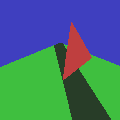
\includegraphics[width=\linewidth]{./imgs/output2}
\caption{}
\label{fig:output2}
\end{wrapfigure}

\begin{wrapfigure}{l}{.8\linewidth}
\centering
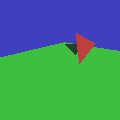
\includegraphics[width=\linewidth]{./imgs/output3}
\caption{}
\label{fig:output3}
\end{wrapfigure}

\begin{wrapfigure}{l}{.8\linewidth}
\centering

\includegraphics[width=\linewidth]{./imgs/output4}
\caption{}
\label{fig:output4}
\end{wrapfigure}

\end{multicols}

It can be seen that the sky acts as a uniform light plane and the triangles at different locations and sizes cast shadows
onto the ground.

\section{Personal Contribution}

\section{Conclusion}
In this project, we have created a method with which to model light rays reflecting off of a surface, including shadows. We also
included the potential for different colors and shades, based on what you want the material to reflect. We have included the capability
for a sky and ground, based on the way which the rays that did not reflect off of anything, sky being angled upwards, and ground
being angled down. Additionally, the 3D rendering system outlined in this report is very modular and could be extended easily to
do things like having the camera follow a path or track certain elements throughout the simulation, allowing for full 360 degree
view of the field.

The code used to complete this assignment is attached as an appendix to this document.

\section{References}
\begin{lstlisting}
https://www.scratchapixel.com/lessons/3d-basic-rendering/ray-tracing-rendering-a-triangle/
                ray-triangle-intersection-geometric-solution

https://en.wikipedia.org/wiki/Pinhole_camera_model
\end{lstlisting}

\newpage
\onecolumn
\section{Appendix}
\lstinputlisting[language=c]{../src/main.c}
\lstinputlisting[language=c]{../src/renderer.c}
\lstinputlisting[language=c]{../src/triangleSurface.c}
\end{document}
